\documentclass[nobib]{tufte-handout} % nobib to have normal citation behaviour 

\usepackage{amsmath, amsthm, amssymb}
\usepackage{xcolor} %for heading colors
\usepackage{titling}
\usepackage{thmtools}
\usepackage[linesnumbered,ruled,vlined]{algorithm2e} %For pseudocode

\usepackage{natbib}
\setcitestyle{authoryear}
%For plots
\usepackage{pgfplots}
\pgfplotsset{compat = newest}

\newtheoremstyle{mytheoremstyle}
    {6pt} % space above
    {6pt} % space below
    {\normalfont} % body font
    {} % indent amount
    {\bfseries} % theorem head font
    {.} % punctuation after theorem head
    {1em} % space after theorem head
    {\thmname{#1}\thmnumber{ #2}\thmnote{ (#3)}} % theorem head spec

\newtheoremstyle{corlstyle}
    {6pt} % space above
    {6pt} % space below
    {\normalfont} % body font
    {} % indent amount
    {\textit{}} % theorem head font
    {.} % punctuation after theorem head
    {1em} % space after theorem head
    {\thmname{#1}\thmnumber{ #2}\thmnote{ (#3)}} % theorem head spec

% Define the theorem environment
\declaretheorem[style=mytheoremstyle,name=Theorem,numberwithin=section]{theorem}

% Define the corollary environment linked to the theorem
\declaretheorem[style=corlstyle,name=Corollary,numberlike=theorem,parent=theorem]{corollary}

\declaretheorem[style=corlstyle,name=Remark,numberlike=theorem]{remark}

\declaretheorem[style=corlstyle,name=Example,numberlike=theorem]{example}

% Define the lemma environment linked to the theorem
\declaretheorem[style=mytheoremstyle,name=Lemma,numberlike=theorem]{lemma}

% Define the proposition environment linked to the theorem
\declaretheorem[style=mytheoremstyle,name=Proposition,numberlike=theorem]{proposition}

% Define the definition environment linked to the theorem
\declaretheorem[style=mytheoremstyle,name=Definition,numberlike=theorem]{definition}

\newcommand\sol{%
  \\ 
  \\
  \textit{Solution:}\\%
}

% --- shortcuts --- %
\newcommand{\indep}{\perp \!\!\! \perp}
\DeclareMathOperator{\var}{Var}
\DeclareMathOperator{\cov}{Cov}
\DeclareMathOperator{\net}{net}

%\geometry{showframe} % display margins for debugging page layout

\usepackage{graphicx} % allow embedded images
  \setkeys{Gin}{width=\linewidth,totalheight=\textheight,keepaspectratio}
  \graphicspath{{graphics/}} % set of paths to search for images

\usepackage{booktabs} % book-quality tables
\usepackage{units}    % non-stacked fractions and better unit spacing
\usepackage{multicol} % multiple column layout facilities
\usepackage{lipsum}   % filler text
\usepackage{fancyvrb} % extended verbatim environments
  \fvset{fontsize=\normalsize}% default font size for fancy-verbatim environments
%\begin{marginfigure}
%  \includegraphics{nonConvex}
%  \label{ConvexExamples2015}
%  \caption{A nonconvex function does not lie below all of its secants.}
%\end{marginfigure}


\usepackage{hyperref}% for better handling of links 

% Prints a trailing space in a smart way.
\usepackage{xspace}

%---- Code ----%
\usepackage{listings}
\usepackage{xcolor}
\definecolor{codegreen}{rgb}{0,0.6,0}
\definecolor{codegray}{rgb}{0.5,0.5,0.5}
\definecolor{codepurple}{rgb}{0.58,0,0.82}
\definecolor{backcolour}{rgb}{0.95,0.95,0.92}
\lstdefinestyle{mystyle}{
    backgroundcolor=\color{backcolour},   
    commentstyle=\color{codegreen},
    keywordstyle=\color{magenta},
    numberstyle=\tiny\color{codegray},
    stringstyle=\color{codepurple},
    basicstyle=\ttfamily\footnotesize,
    breakatwhitespace=false,         
    breaklines=true,                 
    captionpos=b,                    
    keepspaces=true,                 
    numbers=left,                    
    numbersep=5pt,                  
    showspaces=false,                
    showstringspaces=false,
    showtabs=false,                  
    tabsize=2
}
\lstset{style=mystyle}
%/---- Code ----/%
\setcounter{secnumdepth}{4} %to set the section numbering

\newsavebox{\titleimage}
\savebox{\titleimage}{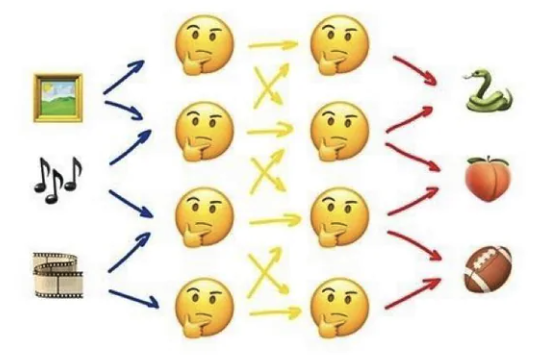
\includegraphics[height=15\baselineskip]{cover.jpg}}

\makeatletter
\renewcommand{\maketitlepage}{%
\begingroup%
\setlength{\parindent}{0pt}

{\fontsize{24}{24}\selectfont\textit{\@author}\par}

\vspace{1.75in}{\fontsize{36}{54}\selectfont\@title\par}

\vspace{0.5in}{\fontsize{14}{14}\selectfont\textsf{\smallcaps{\@date}}\par}

\vspace{0.5in}\usebox{\titleimage}

\vfill{\fontsize{14}{14}\selectfont\textit{\@publisher}\par}

\thispagestyle{empty}
\endgroup
\newpage
}
\makeatother
% Book metadata
\title{An Introduction to Machine Learning}
\date{\today}
\author{Alexandre St-Aubin}
\publisher{McGill University -- Directed Reading Program}

\begin{document}

\maketitlepage% this prints the handout title, author, and date

% r.5 contents
\tableofcontents
\newpage

\section{Introduction}
There are several types of Machine Learning algorithms. The main categories are divided into \textit{Supervised learning, Semi-supervised learning, Unsupervised learning and Reinforcement learning.} Here, we will focus on \textit{Supervised learning.}

\text{\color{red} Introduce problems requiring machine learning, why it is so popular,}

\text{\color{red}what's the goal. How ML is not about understanding the data but more }

\text{\color{red}about being able to infer about new data.}

\begin{definition}[Supervised Learning]
  In supervised learning, the machine learns through examples. The machine learning algorithm is tasked with developing the strategy for achieving the specified outputs given some input.  To do so, a known dataset is supplied  that contains a set of inputs and associated outputs. The algorithm finds patterns in the data, learns from observations, and makes predictions. At the end of the learning process, the algorithm can be tested on data that is unknown to it, but that the operator knows the answers to, in order to test its accuracy. Then, the algorithm is adjusted if needed, and the process continues in an iterated manner.
\end{definition}
\text{\color{red}Types of ML problems (classification, regression).}

\text{\color{red} What is a neural network, quickly talk about components of neural network. }

\text{\color{red} Structure of neural network.}
\section{Neural Networks}
Neural networks, a subset of machine learning, form the core of supervised learning and are inspired by the human brain \citep{web:IBM:NN}.They are made of input, hidden, and output layers, and consist of interconnected \textit{neurons} with associated \textit{weights and thresholds}. Activated nodes transmit data to the next layer if their output surpasses the threshold. 
\subsection{Single Layer Perceptron}%
The simplest neural network is referred to as the perceptron. This neural network contains
a single input layer and an output node \citep{inbook:Aggarwal-1.2}.

Consider a situation where each \textit{training instance} is of the form $(\overline{X}, y)$, where each $\overline{X} = [x_1,..., x_d]$ contains $d$ feature variables, and $y \in [-1, +1]$ contains the observed value of the binary class variable. By “observed value” we refer to the fact that it is given to us as a part of the training data, and our goal is to predict the class variable for cases in which it is not observed.

The input layer of the \textbf{perceptron} contains $d$ nodes that transmit the $d$ features $\overline{X} = [x_1, . . . x_d]$ with \textbf{edges} of \textbf{weight} $\overline{W} = [w_1, . . . w_d]$  to an output node. The input \textbf{layer} does not perform any computation in its own right. The linear function $\overline{W} \cdot \overline{X} =\sum^{d}_{i=1}  w_ix_i$ is computed at the output node. Subsequently, the sign of this real value is used in order to predict the dependent variable of $\overline{X}$. Therefore, the prediction $\hat y$ is computed as follows:
\begin{marginfigure}
  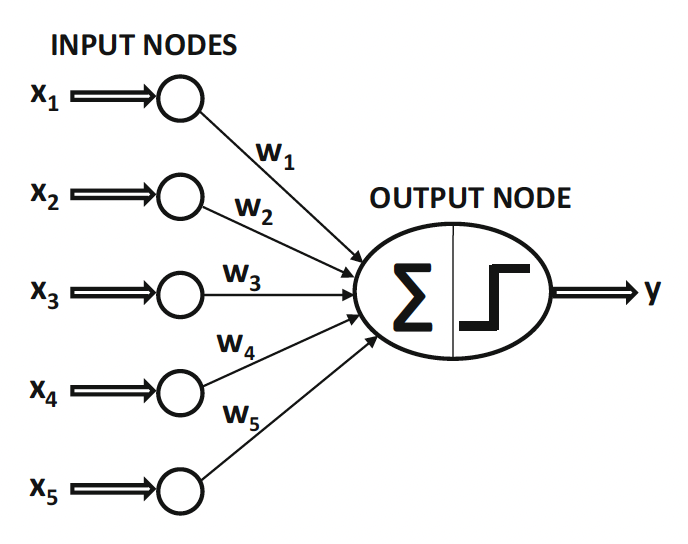
\includegraphics{SingleLayerP}
  \label{SingleLayerP}
  \caption{A single layer perceptron.}
\end{marginfigure}
  \label{sub:Single Layer Perceptron}
 $$\hat y = \text{sign}[\overline{X} \cdot \overline{W}] =\text{sign}\left[\sum^{d}_{i=1}  w_ix_i\right] $$ 
 Here, the sign function serves the role of an activation function (\ref{sub:ActivationFunction}). The goal of the \textbf{perceptron} algorithm with respect to all training instances in a data set $\mathcal{D} = \{(\overline{X_1}, y_1 ), \cdots,(\overline{X_n}, y_n )\}$ is to minimize the loss function (\ref{sub:Loss Function}). We shall learn more about loss functions in a following section, but an example would be to minimize the least-squares function: 
 \begin{equation*}
  \begin{split}
    \sum^{n}_{i=1} (\hat y_i - y_i)^2 =\sum^{n}_{i=1} \left(\text{sign}[\overline{X_i} \cdot \overline{W}] -y_i \right)
  \end{split}
 \end{equation*}
 To optimize the loss function, the perceptron will use a \textit{gradient descent} method, which we will see later.
 \subsection{Neurons}%
  \label{sub:Neurons}
The neuron is the smallest computational unit of a neural network. The single layer perceptron described in the previous section is exactly a neuron.  
\begin{definition}[Neurons]
  Neurons are made up of 4 elements: 
  \begin{enumerate}
    \item The inputs, seen as \textit{nodes}, consist of either the input layer, or the outputs of the previous layer of the neural network. 
    \item The weights and bias, seen as \textit{edges} will act on the inputs before they reach the input function of the neuron. 
    \item The input function takes a sum of the weighed inputs. 
    \item The activation function acts on the input function and outputs the result to the following layers. 
  \end{enumerate}
   receive an input, multiply it by a weight, and output it using an activation function. A simple mathematical model for a neuron's output activation is \citep{book:AIModernApp}
\begin{marginfigure}
  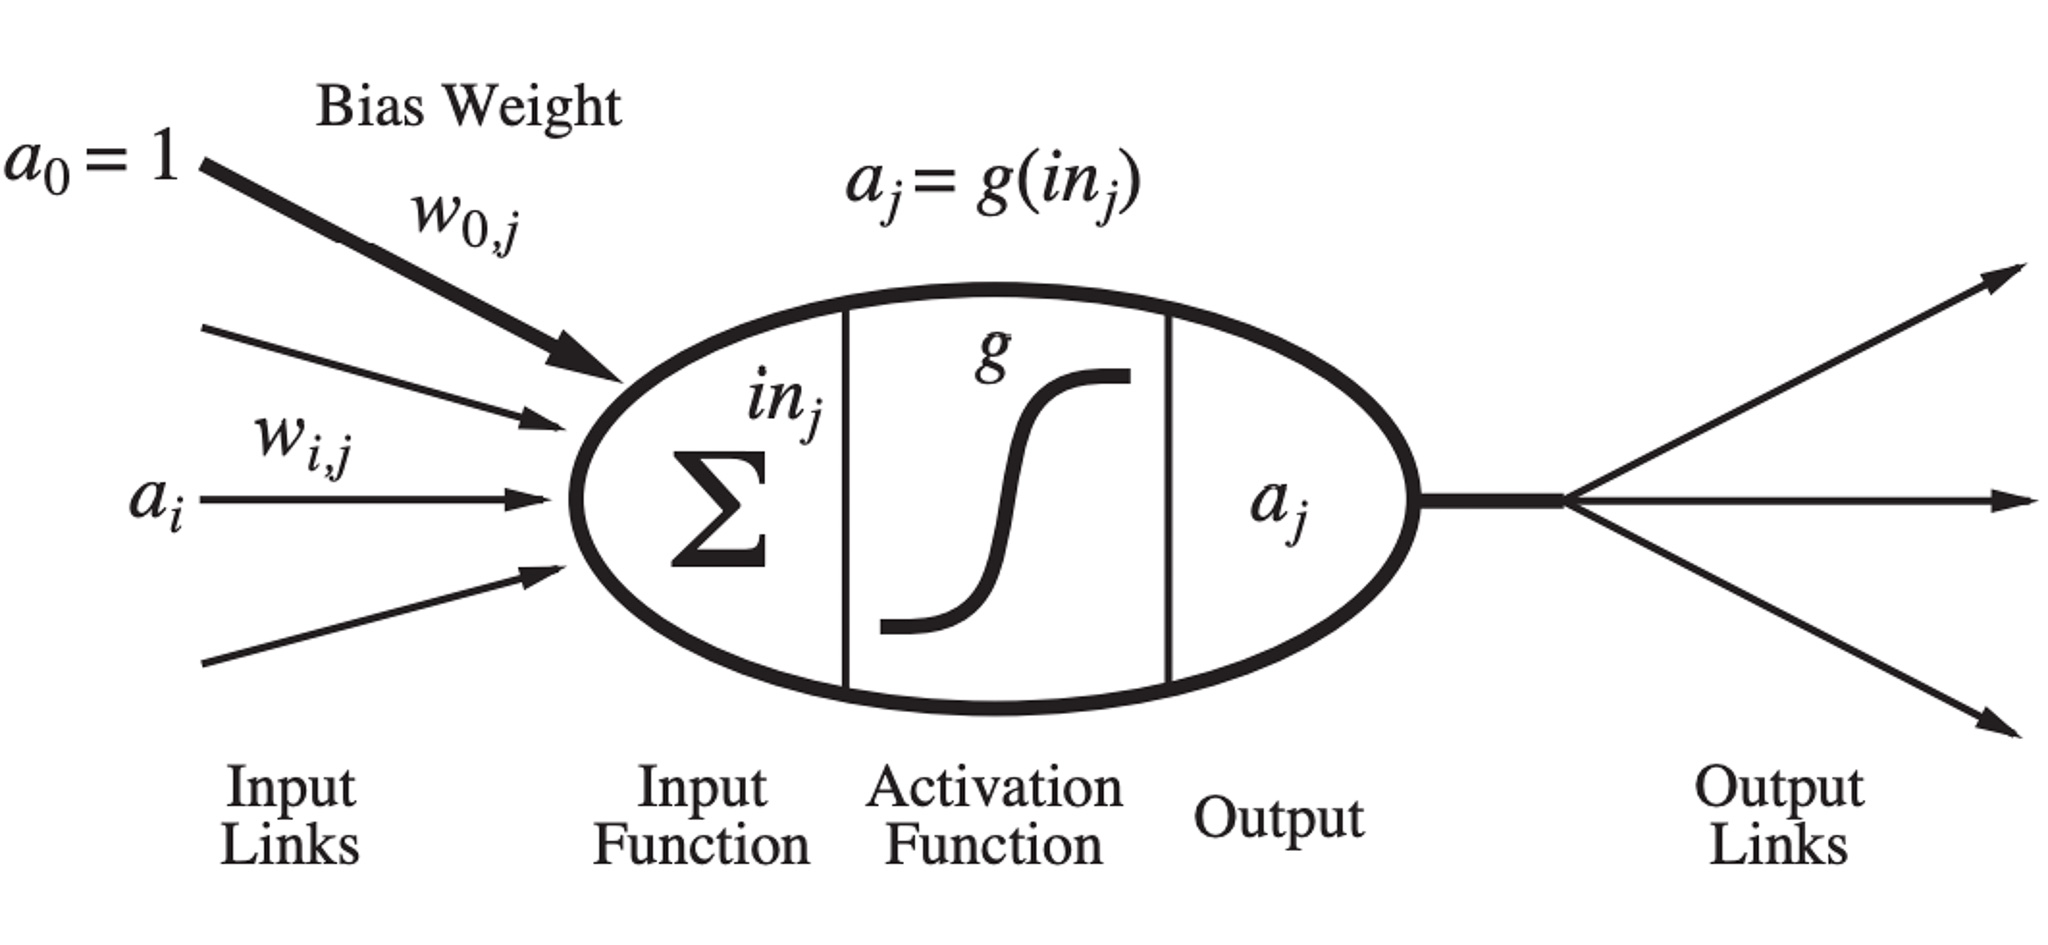
\includegraphics{Neuron}
  \label{Neuron}
  \caption{A neuron and its inputs and outputs.}
\end{marginfigure}
  $$o_j = f \left( \sum^{n}_{i=0}w_{i,j} o_i  \right)$$
  where $f$ is the activation function (\ref{sub:ActivationFunction}), $o_i$ is the output activation of neuron $i$ and $w_{i,j}$ is the weight on the directed edge from neuron $i$ to the neuron $j$. We will explore activation functions in more depth shortly.  
\end{definition}
\begin{definition}[Weights]
  \text{\color{red} FIND A DEFINITION (maybe relate it to the edge of a graph)}
\end{definition}
\subsection{Feed-Forward Neural Networks}%
  \label{sub:Feed-Forward Neural Networks}
  Having defined neurons, the building blocks of neural networks, we may now give a rigorous definition of the latter. A feed-forward network has connections only in one direction—that is, it forms a directed acyclic graph. Every node receives input from “upstream” nodes and delivers output to “downstream” nodes; there are no loops. A feed-forward network represents a function of its current input; thus, it has no internal state other than the weights themselves \citep{book:AIModernApp}.

The overall network is a combination of function composition and matrix multiplication:

  $$g(x) = f^L (W^Lf^{L-1}(W^{L-1} \hdots f^1(W^1x)\hdots)), $$
  where $L$ is the number of layers (\ref{sub:Layers}), $W$ is the weight matrix, and $f$ is the activation function (\ref{sub:ActivationFunction}).
 \begin{definition}[Feed-forward Neural Network]
  A neural network is a \textit{computational directed acyclic graph,} in which a unit of computation is the neuron. Each directed edge in the graph represents a function passing the weighed output of a node in a layer to a node in the next layer.
 \end{definition} 

   Artificial neural networks are often refered to as \textbf{multi-layer perceptrons} (abbreviated to MLPs) for one simple reason: you can think of such an MLP as the composition of multiple perceptrons, where, in this case, the perceptron would be a synonym for artificial neuron, so the smallest computational unit of a neural network, which performs, for example, a linear combination of its inputs followed by the application of an activation function, which can be the sigmoid, tanh, ReLU, identity, or any other function that is differentiable, if you plan to train the neural network with gradient descent.
\subsection{Layers}
\label{sub:Layers}
Feed-forward networks are usually arranged in layers, such that each unit receives input
only from units in the immediately preceding layer. The layers are divided in 3 groups: the \textit{input, hidden,} and \textit{output} layers. See figure \ref{NeuralNetwork} for an image of the layers. Layers are a general term given to a grouping of neurons that act together in the neural network.
\begin{marginfigure}
  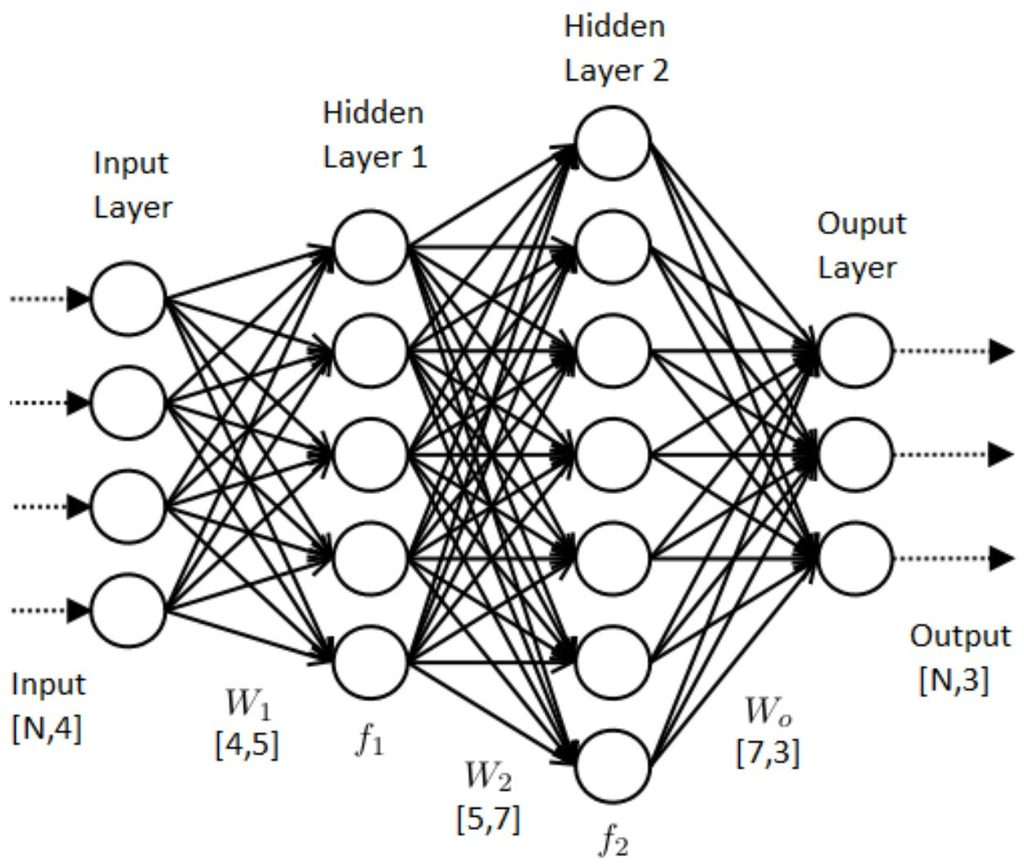
\includegraphics{NeuralNetwork}
  \label{NeuralNetwork}
  \caption{A graph representation of a Neural Network.}
\end{marginfigure}
\begin{definition}[Layers] $  $
  \begin{enumerate}
    \item[\it Input Layer.] The first layer in a neural network, it receives the initial data for the network from the outside world. The "Entry point" of the neural network.
    \item[\it Hidden layers.] The hidden layer(s) are where the magic happens in neural networks. Each layer is trying to learn different aspects about the data by minimizing the \textbf{cost function}. The most intuitive way to understand these layers is in the context of image recognition such as a face. The first layer may learn edge detection, the second may detect eyes, third a nose, etc. \citep{layers}.
    \item[\it Output Layer.] The final layer in the neural network is the output layer. This layer is responsible for holding the final result or output of the problem. Input, such as raw images, is fed into the input layer, and the output layer produces the corresponding result.
\end{enumerate}

\end{definition}

\subsection{Activation Function}%
  \label{sub:ActivationFunction}
An activation function in neural networks is a smooth function applied to the output of each neuron in a layer. It introduces non-linearity to the network, allowing it to learn complex patterns and relationships in the data.

The activation function determines whether a neuron should be activated or not based on the weighted sum of its inputs. In other words, it defines the output of a neuron given a set of inputs. Without activation functions, neural networks would be limited to linear transformations, and they wouldn't be able to capture the non-linearities present in many real-world datasets. 

\vspace{5mm}
\noindent \textbf{Desired Characteristics of Activation Functions} \citep{jagtap2022important}

\noindent There is no universal rule for choosing the best activation function, but there are some characteristics to look for, namely
\begin{enumerate}
  \item[\it Nonlinearity] One of the most essential characteristics
of an activation function is nonlinearity. In comparison
to linear activation functions, the non-linearity of the
activation function significantly improves the learning
capability of neural networks. 
\item[\it Computationally Cheap] The activation function must
be easy to evaluate in terms of computation. This has
the potential to greatly improve network efficiency.
\item[\it Finite Range/Boundedness] Gradient-based training approaches are more stable when the range of the activation function is finite, because pattern presentations
significantly affect only limited weights. 
\item[\it Differentiability] The most desirable quality for using
gradient-based optimization approaches is continuously
differentiable activation functions. This ensures that the
back-propagation algorithm works properly. 
\end{enumerate}
\begin{remark} 
  The vanishing and exploding gradient problems: The variation
of the inputs and outputs of some activation functions,
such as the logistic function (Sigmoid), is extremely
large. To put it another way, they reduce and transform
a bigger input space into a smaller output space that
falls between [0,1]. As a result, the back-propagation
algorithm has almost no gradients to propagate backward
in the network, and any residual gradients that do exist
continue to dilute as the program goes down through the
top layers. Due to this, the initial hidden-layers are left
with no information about the gradients. For hyperbolic
tangent and sigmoid activation functions, it has been
observed that the saturation region for large input (both
positive and negative) is a major reason behind the
vanishing of gradient. One of the important remedies
to this problem is the use of non-saturating activation
functions, such as ReLU.
\end{remark}
We present some commonly used activation functions.
\begin{enumerate}
  \item[\bf Sigmoid Function.] Its range is $[0,1]$, and is defined as,
$$\sigma(x) = \frac{1}{1 + e^{-x}}$$
Advantage: boundedness. \\ Disadvantages:
the vanishing gradient problem, the output not being zerocentered, and the saturation for large input values. 
  \item[\bf Hyperbolic Tangent Function.] It is mostly used for
regression problems, has a range of $[-1,1]$, and is defined as,
$$\tanh(x) = \frac{e^{x} - e^{-x}}{e^{x} + e^{-x}}$$
Advantage: zerocentered structure. \\
Disadvantage: the vanishing gradient problem, i.e. once saturated, it is really challenging
for the learning algorithm to adapt the parameters and learn
faster.
  \item[\bf ReLU Function.] ReLU was primarily used to overcome the vanishing gradient problem. ReLU is the most common activation function used for \textit{classification problems}. Its range is $[0, \infty)$, and is defined as
  $$\text{ReLU}(x) = \max(0, x)$$
Advantages: Apart from overcoming the vanishing gradient problem, the
implementation of ReLU is very easy and thus cheaper, unlike
tanh and sigmoid, where an exponential function is needed.
\\
Disadvantages: It has a saturation region, which can prevent the
learning of the networks. In particular, ReLU always discards
the negative values, which makes the neurons stop responding to
the gradient-based optimizer. This problem is known as \textit{dead
or dying ReLU problem}, meaning the neurons stop
outputting other than zero. 
\item[\bf Softplus Function.] It approximates the ReLU activation function in a smooth way, with a range of $(0, \infty)$, and it is defined as
$$\text{Softplus}(x) = \ln (1+ e^x) $$
\item[\bf Softmax] It is a generalization of logistic
function in high dimensions. It normalizes the output and
divides it by its sum, which forms a probability distribution. The standard softmax function Softmax$: \mathbb{R}^k \to (0,1)^k$ is defined as 
$$\text{Softmax}(x_i) = \frac{e^{x_i}}{\sum^{k}_{j=1} e^{x_j}} \quad \text{for } i= 1,...,k   $$
In other words, it applies
the standard exponential function to each element $x_i$
of the input vector $x$ and normalizes these values by
dividing them by the sum of all these exponentials, which ensures that the sum of the components of the output vector is 1.

\end{enumerate}
The following is a table summarizing the information above. \begin{figure*}
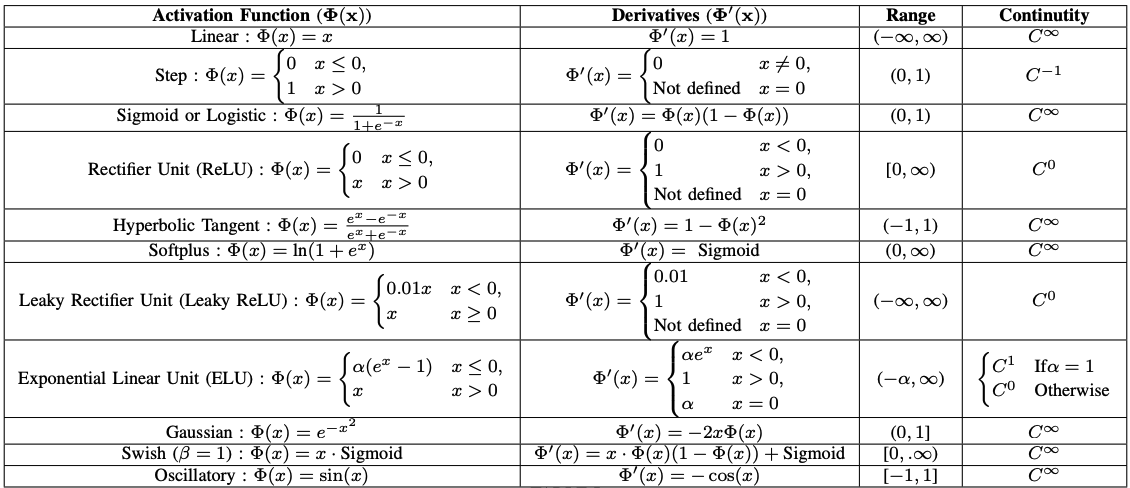
\includegraphics{ActFunTable}
\caption{Common activation functions, their derivatives, range, and order of continuity.}
\end{figure*}

\newpage
\section{Learning}
  \label{sec:Learning}
\subsection{Loss Function}%
  \label{sub:Loss Function}
  Here, we present some common loss functions \citep{ciampiconi2023survey}.
\subsection{BackPropagation}%
  \label{sub:BackPropagation}
\textbf{Backpropagation} is a gradient estimation method used to train neural network models. The gradient estimate is used by the optimization algorithm to compute the network weight updates. So, when we say a neural network is \textit{learning}, it means that backprop is computing a gradient descent that minimizes the loss function, and updates the weights using a \textbf{weight update rule} \ref{sub:Weight Update Rule}. Backpropagation is a way of computing the partial derivatives of a loss function with respect to the weights of a network; we use these derivatives in gradient descent, exactly the way we would with linear regression and logistic regression. 
\begin{marginfigure}
  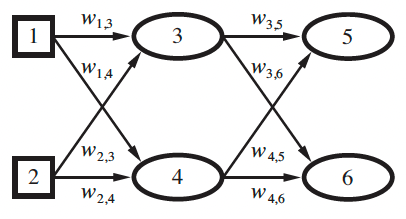
\includegraphics{simpleNet}
  \label{simpleNet}
  \caption{A simple network with 2 inputs, one hidden layer, and two outputs.}
\end{marginfigure}

  Let us first begin by recalling that a neural network evaluates compositions of functions computed at individual nodes. Think of a neural network as a function $h_w(x)$ of the input, parametrized by the weights. Consider the network in Figure \ref{simpleNet}, let $\{x_1,x_2\}$ be the input vector, $f$ the activation function and $a_i$ denote the activated output at node $i$. Then, the output at node 3 is given by
  $$a_3 = f(w_{0, 3} + f(x_1)w_{1,3} + f(x_2)w_{2,3}), $$
  where $w_{0,3}$ is the bias weight at node 3 \text{\color{red}(explain what a bias weight is)}. Similarly, the output at node 5 is
  \begin{equation*}
    \begin{split}
      a_5 &= f( w_{0,5} + f(a_3) w_{3,5} + f(a_4) w_{4,5}  )\\ 
      &= f[w_{0,5} + f(w_{0, 3} + f(x_1)w_{1,3} + f(x_2)w_{2,3})w_{3,5} +f(w_{0, 4} + f(x_1)w_{1,4} + f(x_2)w_{2,4})w_{4,5} ]
    \end{split}
  \end{equation*}
  And even with such a small network, we can already see how awkward it would be to compute the derivative of $a_5$ with respect to $w$. But an even bigger problem arises when we think of how we would compute the loss function in hidden layers. Whereas the error $y -h_w$\sidenote{$y$ is the target output, and $h_w$ the value computed by the network } at the output layer is clear, the error at the hidden layers seems mysterious because the training data do not say what value the hidden nodes should have.

  Therefore, we need some kind of iterative approach to compute the derivatives, and a way to \textit{back-propagate} the error from the output layer to the hidden layers. The resulting iterative approach uses \textit{dynamic programming}, and the \textbf{weight update rule} is the \textit{chain rule} of differential calculus \citep{inbook:Aggarwal-3.2}.

\text{\color{red} continue from p.733 of Russel, p.570 of Murphy, and p.109 of Charu}
\begin{theorem}[Multivariate Chain Rule] \label{chain}
    Let $z = f(y_1, y_2, \ldots, y_m)$ be a differentiable function of $m$ variables, where each $y_j = g_j(x_1, x_2, \ldots, x_n)$ is a differentiable function of $n$ variables. Then, for each $i = 1, 2, \ldots, n$, the partial derivative of $z$ with respect to $x_i$ is given by
$$
\frac{\partial z}{\partial x_i} = \sum_{j=1}^{m} \frac{\partial z}{\partial y_j} \frac{\partial y_j}{\partial x_i}.$$
  \end{theorem}
  We note that backpropagation can be implemented by using either the \textit{pre-activation}, or \textit{post-activation} values at each neuron. Here, we'll focus on the method that acts on the pre activation values neurons. For the sake of simplicity, we view the neural network as a \textit{Directed Acyclic Graph} $G$, where 
  \begin{marginfigure}
    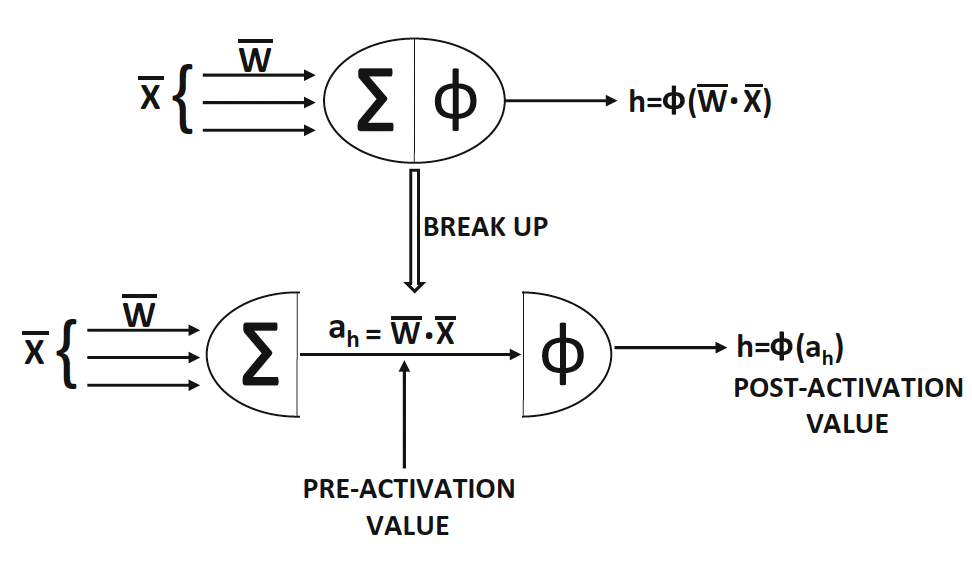
\includegraphics{pre-post-neuron}  
    \caption{Pre and Post activation values of a neuron.}
  \end{marginfigure}
  \begin{enumerate}
    \item Each node represents a neuron, and is denoted by a number $j$.
    \item The weight on the edge from neuron $i$ to $j$ is denoted $w_{i,j}$.
  \end{enumerate}
  The algorithm can be divided in two phases: \textit{forward} and \textit{backward} phases.
  \begin{enumerate}
    \item[\bf Forward Phase.] The term "forward phase" refers to this process of computing values of each hidden layer depending on the current weight values using a specific input vector. These computations naturally cascade forward across the layers. The aim of the forward phase is to compute every intermediate hidden and output variable for a given input. The Backward phase will call for these values. The derivative of the loss function $L$ with respect to this output, as well as the value of the output $o$, are calculated at the completion of the computation. For the sake of simplicity, we will explore the case of a single output node $o$ for the time being. We will then talk about the simple generalisation to many outputs. 

    \item[\bf Backward Phase.] In this phase, the gradient of the loss function with respect to different weights is calculated. First, the derivative $\frac{\partial {o}}{\partial {w}} {}$ is computed. This establishes the gradient computation's initialization. The multivariable chain rule is then used to propagate the derivatives in the opposite direction. Since we are focussing on the pre-activation approach, the gradients are computed with respect to the pre-activation values of the hidden variables, which are then propagated backwards.
  \end{enumerate}
  More precisely, the process can be described as follows. Let $(x,t)$ be the input to our algorithm, where $t$ is the target output of the input vector $x.$ Define the value
  $$L = \operatorname{Loss}(y,t),$$
  where Loss could be any \textit{loss function}, such as the MSE. At each neuron $j$, let its post-activation output be 
  $$o_j = \Phi (\net_j) = \Phi \left( \sum^{n}_{i=0}w_{i,j} o_i  \right) , $$
  where $\Phi$ is any \textit{activation function}, $w_{i,j}$ is the weight on the edge between neurons $i$ and $j$, and $o_i$ is the output from neuron $i.$ Then, the pre-activation value is easily seen to be $\net_j$.

  \begin{enumerate}
    \item The \textbf{forward pass} propagates $x$ through the neural network, computing the values of all hidden neurons to reach the output $\hat y$ of the neural network, which corresponds to the predicted output. Then, $L = \operatorname{Loss}(\hat y, t)$  is computed.
    \item The derivative $\frac{\partial {L}}{\partial {\hat y}}$ at the output can be directly computed. Then, to compute the derivative of $L$ with respect to $o_j$ for an arbitrary neuron $j$, 

    \item Consider $L$ as a function of all neurons receiving input from $j$, and denote this set by $I_j =\{ i_1^{(j)}, ..., i_n^{(j)}\}$. Then, 
    $$\frac{\partial {L(o_j)}}{\partial {o_j}} = \frac{\partial {L(\net_{i_1^{(j)}}, ..., \net_{i_n^{(j)}})}}{\partial {o_j}} {} $$
    to obtain the following recurrence relation for the derivative of $L$ with respect to $o_j$, by the chain rule, 
    \begin{equation}\label{deriv_o_j}
      \begin{split}
        \frac{\partial {L}}{\partial {o_j}} = \mathlarger{\mathlarger{\sum}}^{}_{i \in I_j} \left( \frac{\partial {L}}{\partial {\net_i}} \frac{\partial {\net_i}}{\partial {o_j}}  \right)  =&  \mathlarger{\mathlarger{\sum}}^{}_{i \in I_j} \left( \frac{\partial {L}}{\partial {o_i}} \frac{\partial {o_i}}{\partial {\net_i}} \frac{\partial {\net_i }}{\partial {o_j}} \right) \\ =&\mathlarger{\mathlarger{\sum}}^{}_{i \in I_j} \left( \frac{\partial {L}}{\partial {o_i}} \frac{\partial {o_i}}{\partial {\net_i}} w_{j,i}\right) 
      \end{split}
    \end{equation}
    We can see that the derivative with respect to $o_j$ can be computed if those of the neurons on the next layer are already known, per the \textit{recurrent} behaviour of this algorithm. 
    \item We now have all the necessary tools to compute the partial derivative of $L$ with respect to the weight $w_{i,j}$. Again, by applying the chain rule, we get
    \begin{equation}\label{deriv_w}
  \begin{split}
    {\frac {\partial L}{\partial w_{i,j}}}={\frac {\partial L}{\partial o_{j}}}{\frac {\partial o_{j}}{\partial w_{i,j}}}=&{\frac {\partial L}{\partial o_{j}}}{\frac {\partial o_{j}}{\partial {\text{net}}_{j}}}{\frac {\partial {\text{net}}_{j}}{\partial w_{i,j}}}\\ 
    =& {\frac {\partial L}{\partial o_{j}}}{\frac {\partial o_{j}}{\partial {\text{net}}_{j}}} \left(\frac{\partial {}}{\partial {w_{ij}}} {\sum^{n}_{k=1} w_{k,j}o_k}\right) \\ 
    =&{\frac {\partial L}{\partial o_{j}}}{\frac {\partial o_{j}}{\partial {\text{net}}_{j}}} \left(\frac{\partial {w_{i,j} o_i}}{\partial {w_{i,j}}} \right)={\frac {\partial L}{\partial o_{j}}}{\frac {\partial o_{j}}{\partial {\text{net}}_{j}}} o_i
  \end{split}
\end{equation}
   and so, we may consider the following recursively defined function to simplify notation,

\begin{equation*}
  \begin{split}
    \delta_j = {\frac {\partial L}{\partial o_{j}}}{\frac {\partial o_{j}}{\partial {\text{net}}_{j}}}= 
    \begin{cases}
      \frac{\partial {L(t, o_j)}}{\partial {o_j}} \frac{d {\varphi (\net_j)}}{d {\net_j}}, &\text{ if } j \text{ is an output neuron, }\\
      \left( \sum^{}_{i\in I_j} w_{j,i} \delta_i\right) \frac{d {\varphi (\net_j)}}{d {\net_j}} {}, &\text{ otherwise.} 
    \end{cases}
  \end{split}
\end{equation*}
to conclude that the partial derivative of $L$ with respect to the weight $w_{i,j}$ is given by 
\begin{equation*}
  \begin{split}
    \frac{\partial {L}}{\partial {w_{i,j}}} = o_i \delta_j
  \end{split}
\end{equation*}
      \end{enumerate}
\subsection{Weight Update Rule}%
  \label{sub:Weight Update Rule}
  After having found the derivatives of the loss function with respect to the weights, one needs a way to update the weights. The goal is to modify the weights of the neural network so that given the input $(x,t)$, where $x$ is the input vector and $t$ the target output, it points more toward $t$. Then, in the future, it will have a better chance of classifying $x$ correctly \citep{Hagan_Martin}. The naive way would be to set the weights so that they point directly to $t$. Unfortunately, this leads to overfitting, which we'll address in the next chapter.
  
  To update the weight $w_{i,j}$ using backpropagation, we first choose a learning rate $\mu> 0$. We may then choose to update $w_{i,j}$ by adding $\Delta w_{i,j}$ to it, where
  \begin{equation*}
    \begin{split}
      \Delta w_{i,j} = -\mu \frac{\partial {L}}{\partial {w_{i,j}}}  = - \mu  o_i \delta_j
    \end{split}
  \end{equation*}
 Then, the weight update rule would be defined as, 
 \begin{equation*}
  \begin{split}
    w_{i,j}^{(\text{updated})} =  w_{i,j}^{(\text{old})} - \mu  o_i \delta_j
  \end{split}
 \end{equation*}
 We claim that this update rule decreases the loss $L$. 
 \begin{proof} 
  
If ${\frac {\partial L}{\partial w_{i,j}}}>0$, an increase in $w_{i,j}$ increases $L$; conversely, if $\frac {\partial L}{\partial w_{i,j}}<0$, an increase in $w_{i,j}$ decreases $L$. The new $\Delta w_{i,j}$ is added to the old weight, and the product of the learning rate and the gradient, multiplied by $-1$ guarantees that $w_{i,j}$  changes in a way that always decreases $L$. 
 \end{proof}
  \subsection{Overfitting}%
  \label{sub:Overfitting}
\subsection{Cross-Validation}%
  \label{sub:Cross-Validation}
  
 \section{Example Using Pytorch} 
 \subsection{Introduction}%
  \label{sub:Introduction}
  
In this example, we'll demonstrate how to use PyTorch to implement a Machine Learning model.\cite{brownlee_2023}

\subsection{Importing the Data}
The first step involves preparing and loading your data. Tabular data, such as CSV files, can be handled using common Python libraries. For instance, Pandas facilitates CSV loading, while tools from scikit-learn assist in encoding categorical data like class labels.

PyTorch offers the \texttt{Dataset} class, which permits customization for data loading. Below is a skeletal outline of a custom Dataset class.

\begin{lstlisting}[language=Python, caption=Python code for a PyTorch Dataset class]
class CSVDataset(Dataset):
    # load the dataset
    def __init__(self, path):
        # store the inputs and outputs
        self.X = ...
        self.y = ...
 
    # number of rows in the dataset
    def __len__(self):
        return len(self.X)
 
    # get a row at an index
    def __getitem__(self, idx):
        return [self.X[idx], self.y[idx]]
\end{lstlisting}
Once the data is loaded, PyTorch offers the \texttt{DataLoader} class for navigating a \texttt{Dataset} instance during model training and evaluation. 

The \texttt{random\_split()} function splits a dataset into \textit{train} and \textit{test} sets. After splitting, a subset of rows from the Dataset can be supplied to a \texttt{DataLoader}, along with parameters such as batch size and whether data should be shuffled every \textit{epoch}.

For instance, a \texttt{DataLoader} can be defined by providing a chosen sample of rows from the dataset.
\begin{lstlisting}[language=Python, caption=Python code for creating a DataLoader instance]
...
# create the dataset
dataset = CSVDataset(...)
# select rows from the dataset
train, test = random_split(dataset, [[...], [...]])
# create a data loader for train and test sets
train_dl = DataLoader(train, batch_size=32, shuffle=True)
test_dl = DataLoader(test, batch_size=1024, shuffle=False)
\end{lstlisting}
\subsection{Defining the Model}%
  \label{sub:Defining the Model}
  To define a model in PyTorch we define a class that extends the PyTorch \texttt{Module} class. In the constructor, we will set the layers and the \texttt{forward()} function, which defines the behaviour of the \textit{forward} step of the backprop algorithm.

  In the following code, we define the layers of the NN using the function \texttt{nn.Linear(in, out, bias)}, where \texttt{in} and \texttt{out} represent the size of each input and output sample, respectively. 
\begin{lstlisting}[language=python]
  # model definition
class MLP(Module):
    # define model elements
    def __init__(self, n_inputs):
        super(MLP, self).__init__()
        # define the layers
        self.layer = Linear(n_inputs, 1)
        # define the activation function 
        self.activation = Sigmoid()
 
    # forward propagate input
    def forward(self, X):
        X = self.layer(X)
        X = self.activation(X)
        return X
  \end{lstlisting}
\newpage
    \bibliographystyle{plainnat}
\bibliography{ML_Report_DRP2024}
  
\end{document} 
